\section{Equations Ladder}
\label{sec:eq}


\subsection{Gestion des lampes \textit{En service} et \textit{Hors-service}}
\label{sec:gestion-led}

\underline{\textbf{Énoncé :}} \guillemotleft \ \textit{La lampe} Q2, \textbf{En service}, \textit{est allumée par le poussoir} \textbf{Start}, I4, \textit{et est éteinte par un des défauts non acquitté} (Q1 ou Q8) \textit{ou par l'action sur la commande} \textbf{Stop}.\\
\textit{La lampe} \textbf{Hors service} \textit{est activée quand la lampe} \textbf{En service} \textit{est éteinte}. \guillemotright \

\subsubsection{Équation n°1- Allumer LED Q2 \textit{(En service)}}
\label{sec:eq1}

Lorsqu'on active le bouton poussoir \textbf{Start}, I4, on allume Q2.

\begin{figure}[ht]
  \centering
  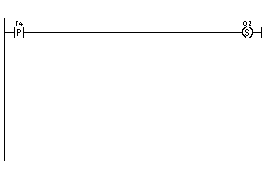
\includegraphics[scale=1.8]
  {textures/images/equations/eq1.pdf}
  \caption{Équation n°1}
  \label{fig:eq1}
\end{figure}


\subsubsection{Équation n°2- Éteindre LED Q2 \textit{(En service)}}
\label{sec:eq2}

Lorsqu'on active le bouton poussoir I5, que les LED Q1 ou Q8 sont allumées, on éteint Q2.

\begin{figure}[ht]
  \centering
  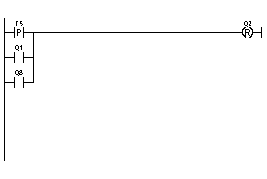
\includegraphics[scale=1.8]
  {textures/images/equations/eq2.pdf}
  \caption{Équation n°2}
  \label{fig:eq2}
\end{figure}


\subsubsection{Équation n°3- Allumer LED Q3 \textit{(Hors-service)}}
\label{sec:eq3}

Si Q2 est éteinte, alors on allume Q3.

\begin{figure}[ht]
  \centering
  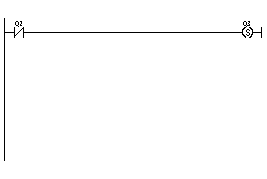
\includegraphics[scale=1.8]
  {textures/images/equations/eq3.pdf}
  \caption{Équation n°3}
  \label{fig:eq3}
\end{figure}


\subsubsection{Équation n°4- Éteindre LED Q3 \textit{(Hors-service)}}
\label{sec:eq4}

SI Q2 est allumée, alors on éteint Q3.

\begin{figure}[ht]
  \centering
  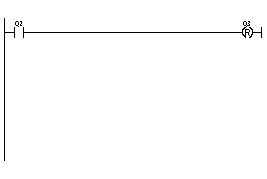
\includegraphics[scale=1.8]
  {textures/images/equations/eq4.pdf}
  \caption{Équation n°4}
  \label{fig:eq4}
\end{figure}

\newpage


\subsection{Gestion des lampes \textit{Défauts moteur}}
\label{sec:gestion-led-defaut}

\underline{\textbf{Énoncé :}} \guillemotleft \ \textit{La présence d'un défaut arrête totalement le fonctionnement de l'installation pour des raisons de sécurité.\\
Les lampes} Q1 \textit{et/ou} Q8 \textit{vont donner les alarmes de défaut liées, respectivement, au} moteur des convoyeurs d'évacuation \textit{et au} moteur principal. \guillemotright \

\subsubsection{Équation n°5- Allumer LED Q1 \textit{(Défaut Moteur des convoyeurs d'évacuation)}}
\label{sec:eq5}

Afin d'allumer la LED Q1, il faut que l'automate soit en service.\\
Il faut aussi que le moteur Q5 soit en surcharge, \textbf{ou}
que l'un des bits mémoires M11 et M12 soit à 1, \textbf{ou}, \textit{c'est un bonus}, que le moteur Q5 soit arrêté, mais qu'une boite passe le détecteur I3.

\begin{figure}[ht]
  \centering
  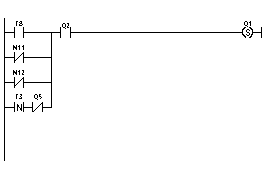
\includegraphics[scale=1.8]
  {textures/images/equations/eq5.pdf}
  \caption{Équation n°5}
  \label{fig:eq5}
\end{figure}


\subsubsection{Équation n°6- Allumer LED Q8 \textit{(Défaut Moteur principal)}}
\label{sec:eq6}

Afin d'allumer la LED Q8 il faut que le moteur Q4 soit en surcharge.

\begin{figure}[ht]
  \centering
  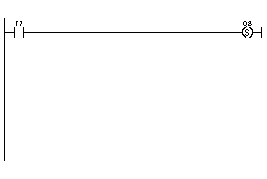
\includegraphics[scale=1.7]
  {textures/images/equations/eq6.pdf}
  \caption{Équation n°6}
  \label{fig:eq6}
\end{figure}

\newpage

\subsubsection{Équation n°7- Éteindre LED Q1 \textit{(Défaut Moteur des convoyeurs d'évacuation)}}
\label{sec:eq7}

Afin d'éteindre la LED Q1, il faut utiliser le \textbf{sélecteur à clé}, I6 \textit{(acquittement)}.

\begin{figure}[ht]
  \centering
  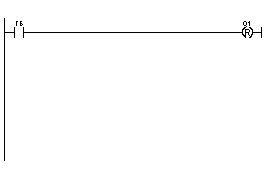
\includegraphics[scale=1.8]
  {textures/images/equations/eq7.pdf}
  \caption{Équation n°7}
  \label{fig:eq7}
\end{figure}


\subsubsection{Équation n°8- Éteindre LED Q8 \textit{(Défaut Moteur principal)}}
\label{sec:eq8}

Afin d'éteindre la LED Q8, il faut utiliser le \textbf{sélecteur à clé}, I6 \textit{(acquittement)}.

\begin{figure}[ht]
  \centering
  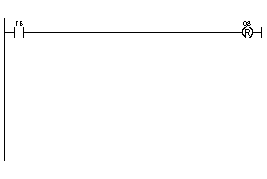
\includegraphics[scale=1.8]
  {textures/images/equations/eq8.pdf}
  \caption{Équation n°8}
  \label{fig:eq8}
\end{figure}

\newpage

\subsection{Encombrement des tapis d'évacuation}
\label{sec:encombrement}

\underline{\textbf{Énoncé :}} \guillemotleft \ \textit{Pour déterminer un encombrement, deux bits mémoires sont utilisés} M11 \textit{et} M12.\\
\textit{Pour} M11 \textit{par exemple, il est activé quand on veut pousser une boite, mais qu'une autre est présente sur le tapis d'évacuation.\\
Il est désactivé quand on a} I13. \guillemotright \

\subsubsection{Équation n°9- Désactivation du bit mémoire M11 \textit{(Vérin A)}}
\label{sec:eq9}

Afin de désactiver le bit mémoire M11 \textit{(bit à 0)}, il faut que I13 ne détecte pas de boite.

\begin{figure}[ht]
  \centering
  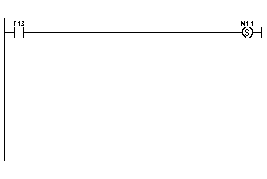
\includegraphics[scale=1.75]
  {textures/images/equations/eq9.pdf}
  \caption{Équation n°9}
  \label{fig:eq9}
\end{figure}


\subsubsection{Équation n°10- Activation du bit mémoire M11 \textit{(Vérin A)}}
\label{sec:eq10}

Pour l'activer \textit{(bit à 1)}, I13 doit détecter un boite et le \textbf{détecteur} I1 doit être en front descendant \textit{(c'est-à-dire qu'une boite détectée sort du champ du détecteur et se retrouve devant le vérin)}.

\begin{figure}[ht]
  \centering
  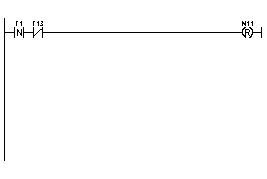
\includegraphics[scale=1.75]
  {textures/images/equations/eq10.pdf}
  \caption{Équation n°10}
  \label{fig:eq10}
\end{figure}

\newpage

\subsubsection{Équation n°11- Désactivation du bit mémoire M12 \textit{(Vérin B)}}
\label{sec:eq11}

Afin de désactiver le bit mémoire M12 \textit{(bit à 0)}, il faut que I14 ne détecte pas de boite \textit{(c'est-à-dire que le tapis d'évacuation n'est pas encombré)}.

\begin{figure}[ht]
  \centering
  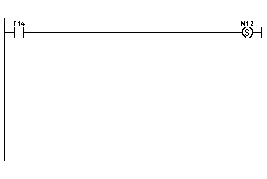
\includegraphics[scale=1.8]
  {textures/images/equations/eq11.pdf}
  \caption{Équation n°11}
  \label{fig:eq11}
\end{figure}


\subsubsection{Équation n°12- Activation du bit mémoire M12 \textit{(Vérin B)}}
\label{sec:eq12}

Pour l'activer \textit{(bit à 1)}, le \textbf{détecteur} I2 doit être en front descendant  et I14 doit détecter un boite.

\begin{figure}[ht]
  \centering
  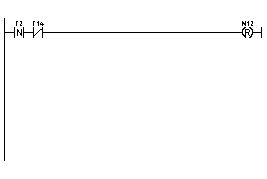
\includegraphics[scale=1.8]
  {textures/images/equations/eq12.pdf}
  \caption{Équation n°12}
  \label{fig:eq12}
\end{figure}

\newpage

\subsection{Gestion des vérins}
\label{sec:verins}

\underline{\textbf{Énoncé :}} \guillemotleft \ \textit{La sortie du vérin s'effectue soit en fin d'encombrement} (il faut pousser la boite encore présente), \textit{soit quand une boite est reconnue et qu'on n'a pas d'encombrement.\\
La tige du vérin doit être rentrée quand on est} Hors-service \textit{ou que la boite est positionnée sur son tapis d'évacuation}. \guillemotright \

\subsubsection{Équation n°13- Activation du moteur Q6 \textit{(Vérin A)}}
\label{sec:eq13}

Pour activer le moteur Q6, il faut que l'automate soit actif.\\
De plus, I1 doit être en front descendant et le bit mémoire M11 doit être à \textit{0}.

\begin{figure}[ht]
  \centering
  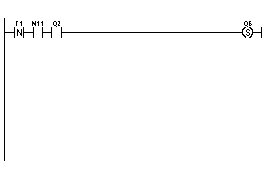
\includegraphics[scale=1.8]
  {textures/images/equations/eq13.pdf}
  \caption{Équation n°13}
  \label{fig:eq13}
\end{figure}


\subsubsection{Équation n°14- Désactivation du moteur Q6 \textit{(Vérin A)}}
\label{sec:eq14}

Pour que le vérin A soit désactivé, il faut que I13 détecte une boite, \textbf{ou} que l'automate soit éteint.

\begin{figure}[ht]
  \centering
  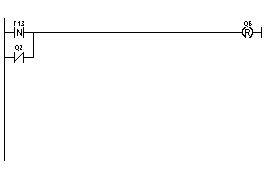
\includegraphics[scale=1.8]
  {textures/images/equations/eq14.pdf}
  \caption{Équation n°14}
  \label{fig:eq14}
\end{figure}

\newpage

\subsubsection{Équation n°15- Activation du moteur Q7 \textit{(Vérin B)}}
\label{sec:eq15}

Pour activer le moteur Q7, il faut que l'automate soit actif.\\
De plus, I2 doit être en front descendant et le bit mémoire M12 doit être à \textit{0}.

\begin{figure}[ht]
  \centering
  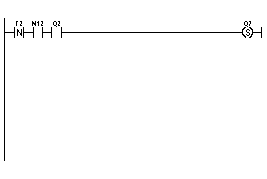
\includegraphics[scale=1.8]
  {textures/images/equations/eq15.pdf}
  \caption{Équation n°15}
  \label{fig:eq15}
\end{figure}


\subsubsection{Équation n°16- Désactivation du moteur Q7 \textit{(Vérin B)}}
\label{sec:eq16}

Pour que le vérin B soit désactivé, il faut que I14 détecte une boite, \textbf{ou} que l'automate soit éteint.

\begin{figure}[ht]
  \centering
  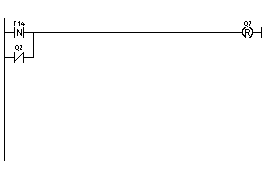
\includegraphics[scale=1.8]
  {textures/images/equations/eq16.pdf}
  \caption{Équation n°16}
  \label{fig:eq16}
\end{figure}

\newpage

\subsection{Gestion des moteurs des convoyeurs}
\label{sec:moteurs}

\underline{\textbf{Énoncé :}} \guillemotleft \ \textit{Le convoyeur principal fonctionne si les vérins sont rentrés, s'il n'y a pas de bourrage et si on est} En service.\\
\textit{Le moteur des tapis d'évacuation est en marche avec le sélecteur et la lampe} En service. \guillemotright \

\subsubsection{Équation n°17- Moteur principal \textit{(Q4)}}
\label{sec:eq17}

Le moteur principal est activé lorsque l'automate est en service et que les deux vérins sont rentrés.

\begin{figure}[ht]
  \centering
  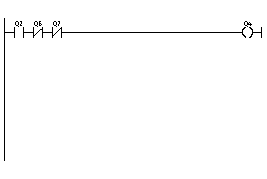
\includegraphics[scale=1.8]
  {textures/images/equations/eq17.pdf}
  \caption{Équation n°17}
  \label{fig:eq17}
\end{figure}


\subsubsection{Équation n°18- Moteur d'évacuation \textit{(Q5)}}
\label{sec:eq18}

Le moteur des convoyeurs d'évacuation est activé si l'automate est activé et que l'\textbf{interrupteur} I17 l'est aussi.

\begin{figure}[ht]
  \centering
  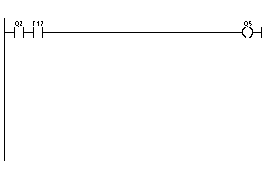
\includegraphics[scale=1.8]
  {textures/images/equations/eq18.pdf}
  \caption{Équation n°18}
  \label{fig:eq18}
\end{figure}

\newpage

\subsection{Gestion des compteurs de boites}
\label{sec:compteurs}

\underline{\textbf{Énoncé :}} \guillemotleft \ \textit{À la détection d'une boite grise par le capteur }I1, \textit{le} Vérin A \textit{pousse la boite sur le} convoyeur d'évacuation.\\
\textit{Un} compteur \textit{s'incrémente, indiquant le nombre de boites.\\
Un} compteur \textit{différent est utilisé pour chaque modèle de boite.\\
De plus, les compteurs doivent se réinitilaliser lors de l'activation du sélecteur à clé} I18. \guillemotright \

\subsubsection{Équation n°19- Compteur de boites \textit{(couleur Argent)}}
\label{sec:eq19}

Le \textbf{compteur} C1, pour les boites argentées, s'incrémente lorsque I13 détecte une boite.\\
Il se réinitialise si l'automate s'éteint, \textbf{ou} qu'on active le \textbf{sélecteur à clé}, I18.

\begin{figure}[ht]
  \centering
  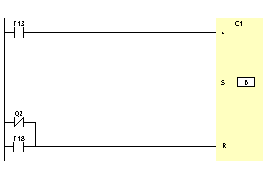
\includegraphics[scale=1.8]
  {textures/images/equations/eq19.pdf}
  \caption{Équation n°19}
  \label{fig:eq19}
\end{figure}


\subsubsection{Équation n°20- Compteur de boites \textit{(couleur Cuivre)}}
\label{sec:eq20}

Le \textbf{compteur} C2, pour les boites cuivrées, fonctionne de la même manière que le compteur C1.\\
La différence est que l'incrémentation est lancée lorsque \textbf{I14} détecte une boite.


\subsubsection{Équation n°21- Compteur de boites \textit{(couleur Or)}}
\label{sec:eq21}

Le \textbf{compteur} C3, pour les boites dorées, fonctionne de la même manière que les compteurs C1 et C2.\\
La différence est que l'incrémentation est lancée lorsque \textbf{I3} détecte une boite.
